\section{NUIssues}

In the previous section, we had a brief look at natural user interfaces as a concept and how it manifests itself in current technology, before presenting the problem this project attempts to answer: how can designing an issue tracker for the natural user interface type \textit{touch} boost productivity?

This section is a presentation of the issue tracker, hereinafter referred to as \textit{NUIssues}.

\subsection{Definitions}

Before entering a presentation of the issue tracking system NUIssues, a common domain language must be established.

\begin{itemize}
  \item \textbf{Issue}: The conceptual, individual task to be completed. Represented graphically by \textit{card}s, which are moved between \textit{swimlane}s as the task's status switches between \textit{todo}, \textit{doing}, and \textit{done}.
  \item \textbf{Card}: A graphical representation of an issue. To be moved between \textit{swimlane}s as the status of the issue changes.
  \item \textbf{Swimlane}: A vertical container for issues to indicate their status. Each issue resides within a single swimlane. NUIssues has three swimlanes along the \textbf{x} axis of the GUI: \textit{todo}, \textit{doing}, and \textit{done}.
  \item \textbf{Index}: Each \textit{card}'s vertical (y axis) position in a \textit{swimlane}, and (by convention) the relative priority of the issue.
\end{itemize}

\subsection{Rationale behind building an issue tracker}

An issue tracker in particular was selected because almost everyone has used a similar system before, be it through clinging Post-It!s to a wall or using digital systems like Trello, Atlassian JIRA, Asana, and Ding.io. This way, the user will already have a mental model for a simple issue tracker, and all focus can be on optimising the mechanics of the application for natural input. The primary goal has been to optimise the actual board interaction for \textbf{touch} input: the \textit{natural} way of moving physical cards around is to touch and drag them.

Importantly, an issue tracker also lends itself to a highly interactive environment where almost everything can be moved to let the user customise the layout. This seems to be optimal conditions for a small proof of concept on touch optimisation.

From a software integration perspective, it is clear that visualising something as integral to an organisation as \textit{tasks} in a clear way that provides quick insight into the state of a project will be very helpful. Given a supportive Application Programming Interface (API), should also be a relatively simple task to integrate the application with existing issue tracking systems in order to provide a more natural interface for managing tasks.

\subsection{Scope and sketch}

NUIssues is a system with a 2D GUI optimised for the Natural User Interface \textbf{touch}. As is to be expected of an issue tracking system, there are no aspects of Augmented Reality (AR), Virtual Reality (VR), or Mixed Reality (MR). These are certainly interesting areas to explore in the future, but not within the scope of this project.

Figure \ref{figure:ipad-mockup} shows a simple initial mockup for the application's main functionality. For comparison, figure \ref{figure:ipad-default-simple-screenshots} shows the implemented, much more refined and informative result.

\begin{figure}[H]
    \centerline{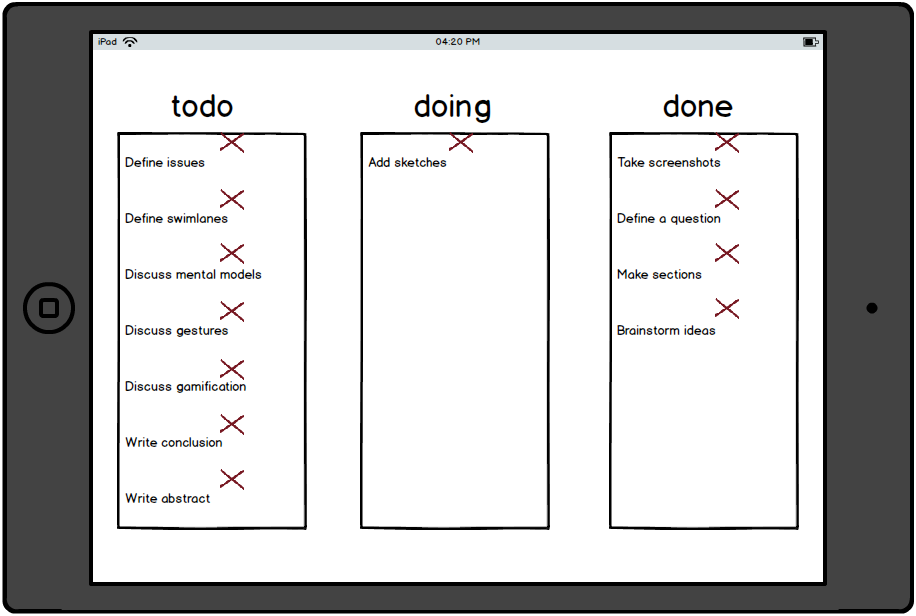
\includegraphics[scale=0.4]{images/mockup}}
    \caption{A simple mockup of the main functionality}   
    \label{figure:ipad-mockup}
\end{figure}

\begin{figure}[H]
    \centerline{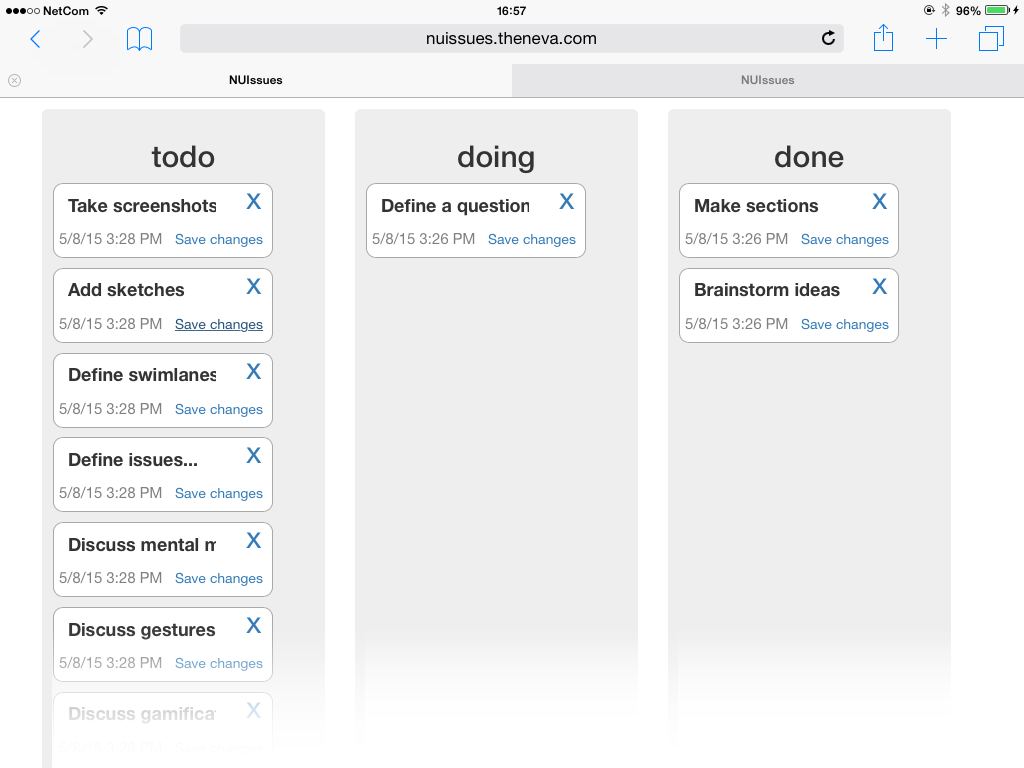
\includegraphics[scale=0.4]{images/nuissues-screenshots/01-default-all-swimlanes}}
    \caption{The system image for the main functionality}
    \label{figure:ipad-default-simple-screenshots}  
\end{figure}

The interface is designed only for Apple iPad 1/2/Mini, but one may easily write responsive CSS to support more types of devices. This allows bringing the very simple interface to natural interfaces like \textit{touch walls}, \textit{touch tables}, in addition to smartphones and desktop computers. The interface is designed to be used when sitting down, although the application can certainly merely be opened if the user's intent is to grok the project's state while on the move.

If the user intends to edit textual content (only the title in NUIssues), it would be preferable to have an external keyboard. As reflected upon in the introduction, a keyboard is by far the most effective tool to write precise text in a computer system. An on-screen software keyboard will work almost as well, but overlaps almost all of the issues. Thus, the application is unusable for anything other than finishing text input and saving changes when in the editing state.

% everything below this point is a draft

Motion controllers, gaze trackers, and brain trackers may be less interesting to use here (although Atlassian has been able to use brain power to move issues between swimlanes at a hackathon – or so they say).

Could have built something native for better performance and complete control of the environment, but takes far too much time and was beside the concept we set out to prove.

Touch input: Fat fingers: no buttons (only large areas), large margins, everything can be dragged (no specific drag handles), may cause trouble with scrolling

While not explicitly expressed, one may assume that the user's model of the system identifies issues higher up (with a lower index) as more important. After all, the grid layout imposes a hierachical style on the application. This interpretation is, however, left to the user.

The system is single-user, so inter-user task coupling has not been explicitly addressed, but it is possible to evolve the system to other forms of interfaces like touch walls or touch tables (or even just real-time updates for a project).

Inter-user task coupling (irrelevant because no two users will use the system at the same time – but could implement this with sockets so that both users will always know what the current status is)

% TODO: Look into socket support for multi-user updates, in which case we probably move to lightly coupled tasks

% TODO: figure out/discuss what type of coupling the tasks of updating an issue tracker are

% TODO: Cost/benefit discussion of different input types, what was NOT implemented

% TODO: Discuss fingerprint login (TUI!) and ethical issues with identifying someone/storing that type of information

Ethical problems: none in this application (except for security, duh), but certainly applicable % TODO: Digress into short discussion of ethical issues generally raised in NUI/Interactive Technologies contexts, especially fingerprint identification/login (see Apple's model of fingerprint "storage")

Gamification: no users (and no points)\dots % TODO: look into and discuss how gamification could be utilised in a task tracker (public scoreboards, points, badges)

\subsection{Mental models in NUIssues}

\textcite{wilson-rutherford:mental-models-theory-and-application-in-human-factors:1989} introduces the notion of \textit{mental models} within Human-Computer Interaction (HCI), defined as any human's psychological representation (and implied expectations for) any given concept or object. A person will build a mental model for themselves, and for any object they interact with. They introduce a framework for the design phase of any computer system, with four distinctly different models at play.

First, one needs to define a \textit{target system}. In this case, the target system is the NUIssues system and interface.

Second, there is a \textit{conceptual model}, which is a very accurate psychological representation of exactly what the system does, usually held by an expert user or the designer themselves.

Fourth, the target system projects a \textit{system image}, which is the implementation of the the conceptual model. This is the basis for the next element: the user's mental model of the system.

Fifth, the \textit{user} immediately builds a mental model of the system of the system based on the \textit{system image}. This model is the basis for what the user expects the system to be able to do, mostly based on previous experience with similar systems but only based on the hints given by the application.

Last, the \textit{designer has a mental model of the user's model}, in which the designer attempts to guess what the user's mental model of the system image will be like. This model is built on the target audience's expected background, and can be built by considering similar applications the user can be expected to have interacted with in the past. In this case, an obvious system is that of sticky notes and checklists to track tasks, which almost everyone has used at some point. Thus, these graphical representations of issues may be used as metaphors in the system. Further, the user can have come across several digital issue trackers optimised for web like \footnote{\url{https://trello.com}}, Atlassian JIRA\footnote{\url{https://jira.atlassian.com/secure/Dashboard.jspa}}, Ding\footnote{\url{https://ding.io}}, ServiceNow\footnote{\url{http://www.servicenow.com/}}, and IBM Notes\footnote{\url{http://www-03.ibm.com/software/products/en/ibmnotes}}.

\subsection{Behaviour models}

Hick-Hyman Law: about reaction time when presented with a bunch of options, not really relevant as there are zero menus (for which the law is mostly being used)

Keystroke-level model (KLM): Key stroking only relevant when adding or editing issues, pointing relevant because the finger moves, homing time minimised because of large, responsive controls, drawing minimised (and destinations hinted), mental operator, system response operator (hello Heroku) % TODO look into mental operator and System Response operator

Motor behaviour models: descriptive models: (state 0: waiting for stimuli) -> <finger down on issue handle (entire issue)> -> ((state 1: dragging issue) -> <finger up above legal area> -> (state 2: releasing "dropping" issue) -> (state 0: waiting for stimuli)) OR (<finger up from text> -> (state 4: editing text) -> <tap "save changes" control> -> (state 0: waiting for stimuli))

\subsection{Development process}

Web client can be used by all types of devices (phones, tablets, touch tables, "smartboards", touch walls)

No specific SDKs have been used, although several frameworks are used:
\begin{itemize}
  \item AngularJS (front-end) with ng-sortable, bootstrap 3, custom CSS
  \item Node.js (back-end) with several components (Express web server, Mongoose ODM (could just as easily have used relations), body-parser)
  \item MongoDB document database (could just as easily have used relations for this simple use case)
  \item Potential: JWT (or just cookies): save data inside the token
\end{itemize}

\subsection{Known bugs}

\begin{itemize}
  \item It is nearly impossible to grab the bottommost issue that lies beneath the "fade out" overlay over the swimlane in a full swimlane
\end{itemize}
